% 		replace .lof file ========================================================================
%  Copyright (c) 1985-2014 The University of Washington
%
%  Licensed under the Apache License, Version 2.0 (the "License");
%  you may not use this file except in compliance with the License.
%  You may obtain a copy of the License at
%
%      http://www.apache.org/licenses/LICENSE-2.0
%
%  Unless required by applicable law or agreed to in writing, software
%  distributed under the License is distributed on an "AS IS" BASIS,
%  WITHOUT WARRANTIES OR CONDITIONS OF ANY KIND, either express or implied.
%  See the License for the specific language governing permissions and
%  limitations under the License.
%  ========================================================================
%

% Documentation for University of Washington thesis LaTeX document class
% by Jim Fox
% fox@washington.edu
%
%    Revised for version 2015/03/03 of uwthesis.cls
%
%    This document is contained in a single file ONLY because
%    I wanted to be able to distribute it easily.  A real thesis ought
%    to be contained on many files (e.g., one for each chapter, at least).
%
%    To help you identify the files and sections in this large file
%    I use the string '==========' to identify new files.
%
%    To help you ignore the unusual things I do with this sample document
%    I try to use the notation
%       
%    % --- sample stuff only -----
%    special stuff for my document, but you don't need it in your thesis
%    % --- end-of-sample-stuff ---


%    Printed in twoside style now that that's allowed
%
 
\documentclass [11pt, proquest] {uwthesis}[2015/03/03]
 
%
% The following line would print the thesis in a postscript font 

% \usepackage{natbib}
% \def\bibpreamble{\protect\addcontentsline{toc}{chapter}{Bibliography}}

\setcounter{tocdepth}{1}  % Print the chapter and sections to the toc
 

% ==========   Local defs and mods
%

% --- sample stuff only -----
% These format the sample code in this document

\usepackage{alltt}  % 
\newenvironment{demo}
  {\begin{alltt}\leftskip3em
     \def\\{\ttfamily\char`\\}%
     \def\{{\ttfamily\char`\{}%
     \def\}{\ttfamily\char`\}}}
  {\end{alltt}}
 
% metafont font.  If logo not available, use the second form
%
% \font\mffont=logosl10 scaled\magstep1
\let\mffont=\sf
% --- end-of-sample-stuff ---
 
\usepackage{color} 
 
\usepackage{graphicx}
\graphicspath{ {figures/} }

% packages Tyler added
\usepackage{amsmath}
\usepackage{amssymb}
\usepackage{mathrsfs}
\usepackage{subfigure}

\usepackage{caption}
\captionsetup{justification=justified}

\begin{document}
 
% ==========   Preliminary pages
%
% ( revised 2012 for electronic submission )
%

\prelimpages
 
%
% ----- copyright and title pages
%
\Title{Smart Things and Cochlear Implants}
\Author{Tyler Ganter}
\Year{1985-2014}
\Program{UW Information Technology}

\Chair{Name of Chairperson}{Title of Chair}{Department of Chair}
\Signature{First committee member}
\Signature{Next committee member}
\Signature{etc}

% \copyrightpage

% \titlepage  

% --- sample stuff only -----
% unusual footnote not found in a real thesis
% You just use the \titlepage as commented out above

{\Degreetext{A dissertation%
  \footnote[2]{an egocentric imitation, actually}\\
  submitted in partial fulfillment of the\\ requirements for the degree of}
 \def\thefootnote{\fnsymbol{footnote}}
 \let\footnoterule\relax
 \titlepage
 }
\setcounter{footnote}{0}

% --- end-of-sample-stuff ---
 
%
% ----- signature and quoteslip are gone
%

%
% ----- abstract
%


\setcounter{page}{-1}
\abstract{%

This document is about extracting harmonic envelopes, what matters, what doesn't and how to design your system accordingly.  It is broken into three parts:
 
\begin{itemize}
\item envelope extraction techniques and their relationships
\item phase preservation
\item system design (filter and downshift)
\end{itemize}

Many strategies consider the effects of leaving modulations in the signal, but nothing really talks about what the envelope should be, independent of the modulations.  If we do this first, we can than think about how the modulations affect this envelope as a separate modulation component.

If explicitly inducing modulations it is important to remove any other modulations, and this is how.

}
 
%
% ----- contents & etc.
%
\tableofcontents
\listoffigures
%\listoftables  % I have no tables
 
%
% ----- glossary 
%
\chapter*{Glossary}      % starred form omits the `chapter x'
\addcontentsline{toc}{chapter}{Glossary}
\thispagestyle{plain}
%
\begin{glossary}
\item[argument] replacement 
\item[back-up] a copy of a fi
 
\end{glossary}
 
%
% ----- acknowledgments
%
\acknowledgments{% \vskip2pc
  % {\narrower\noindent
  The author wishes to express sincere appreciation to
  University of Washington, where he has had the opportunity
  to work with the \TeX\ formatting system,
  and to the author of \TeX, Donald Knuth, {\it il miglior fabbro}.
  % \par}
}

%
% ----- dedication
%
\dedication{\begin{center}to my dear wife, Joanna\end{center}}

%
% end of the preliminary pages
 
 

%
% ==========      Text pages
%

\textpages
 
% ========== Chapter 1
 
\chapter{Introduction}

this is the introduction

Why harmonic encoding?  Help differentiate signals, (timbre), improve SIN performance, free up channels for other information

\section{Overview}

we are considering what is the ideal matched filter, and how close of an approximation do we need?

\section{Survey of Literature}

Equivalent noise bandwidth (ENBW) considers BW of noise if squished into a box of gain 1 around the downshift frequency.  [windows for harmonic analysis] This isn't entirely applicable since our harmonic has BW > epsilon, and since for any window most of the energy is close to 0, most of the so-called noise is actually desired harmonic signal.  If this were not the case, (I think) rectangular window would be the best, but since it distributes the noise more heavily to higher frequencies away from zero, it is actually worse (higher sidelobes)

``some windows have a high rate of sidelobe decay that allows minimizing the error due to interference. However the steeper the sidelobe decay
the wider the main lobe width and then the worse the minimum resolution bandwidth.'' [An Intelligent FFT-Analyzer with Harmonic Interference Effect Correction and Uncertainty Evaluation]

``For NH listeners, the timbre space was best represented in three dimensions, one correlated with the temporal envelope (log-attack time) of the stimuli, one correlated with the spectral envelope (spectral centroid), and one correlated with the spectral fine structure (spectral irregularity) of the stimuli. The timbre space from CI listeners, however, was best represented by two dimensions, one correlated with temporal envelope features and the other weakly correlated with spectral envelope features of the stimuli. 
``temporal envelope is dominant cue for timbre perception in CI listeners''
[Temporal and Spectral Cues for Musical Timbre
Perception in Electric Hearing]

Hypothesis:
--temporal envelope (log-attack time)
this is in some cases smeared in time (F0mod) and in other cases mixed across harmonics
--one correlated with the spectral envelope (spectral centroid)
this is not as clearly represented as it could be (are we talking about resonance or per-harmonic details such as clarinet?)
--one correlated with the spectral fine structure (spectral irregularity)
this manifests in the envelope for CI processing, the problem though is that it is blurred across harmonics so the noise-like characteristics will be smoothed.

\section{Contents of Thesis}

% ========== Chapter 2

\chapter{Background}

``By definition, timbre is the perceptual attribute that distinguishes two sounds that have the same pitch, loudness, and duration (American National Standards Institute, 1973).''

%\chapter{Envelope Extraction Methods}
%\section{STFT}
%\section{Hilbert}
%\section{CIS}
%\section{Coherent}
%\section{Summary}

\chapter{Harmonic Envelopes}

We model our harmonic signal with a sum-of-products model as:

\begin{align}
\label{eq:sum_of_products}
x[n] = \sum\limits_k x_k[n] = \sum\limits_k m_k[n] c_k[n]
\end{align}

our extracted envelope can be generally defined as:

\begin{align}
\label{eq:envelope_extraction}
%\tilde{m}_k[n] =& \Big| x[n]e^{-j \omega_k\big[F_0[n]\big]n} * h_k\big[n,F_0[n]\big]  \Big| \\
\tilde{m}_k[n] =& \Big| \widehat{x}[n]e^{-j \omega_k[x]n} * h_k[n,x]  \Big|
\end{align}

This is a good generalization of any envelope extraction (harmonic or not). The design can be summarized by two things:

\begin{itemize}
\item downshift frequency, $\omega_k[x]$
\item lowpass filter, $h_k[n,x]$
\end{itemize}

If $w_k[\cdot]$ and $h_k[\cdot]$ are functions of $x[n]$ we have coherent envelope extraction.  If they are time-invariant, we have incoherent extraction.

\subsection{harmonic signals}

Since harmonic signals have a specific structure, we can define our carriers from equation~\ref{eq:sum-of-products} as centered at multiples of $F_0$. In this representation $x_0[n]$ is the fundamental centered at $F_0$, $x_1[n]$ is the 1st harmonic centered at $2F_0$, etc.

\begin{align}
\theta_k[n] =& 2\pi(k+1)\frac{F_0}{F_s}n + \phi_k[n] \\
x[n] =& \sum\limits_{k=0}^K m_k[n] cos(\theta_k[n]) \\
\widehat{x}[n] =& \sum\limits_{k=0}^K m_k[n] e^{j\theta_k[n]}
\end{align}


\section{Steady-State Analysis}

We start with the simplest scenario, where $x[n]$ is a steady-state signal.  The conditions we require for this are:

\begin{itemize}
\item constant pitch: $F_0[n] = F_0$
\item narrowband modulator: $m_k[n] \approx constant$ over short periods of time
\item constant phase term: $\phi_k[n] = \phi_k$, we choose $\phi_k[n] = 0$ for cleaner equations however this is not necessary
\end{itemize}

\subsection{3 Harmonic Example: Desired Envelope}

We visualize the frequency domain for a signal with three harmonics ($K = 2$) in figure~\ref{fig:harmonic_envelope}.  For this example we consider the 1st harmonic ($k = 1$), centered at $2F_0$.

Figure~\ref{fig:harmonic_envelope}$(d)$ is the spectrum of the squared envelope, $| \mathcal{F} \{m_1^2[n] \}|$.  We see this relationship in equation~\ref{eq:harmonic_envelope_spectrum_d}

\begin{align}
\label{eq:harmonic_envelope_spectrum_a}
(a)& \quad \widehat{x}[n] \Longleftrightarrow \widehat{X}[n,f)  \\
(b)& \quad \widehat{x}_1[n] \Longleftrightarrow \widehat{X}_1[n,f) \\
(c)& \quad \widehat{x}_1^*[n] \Longleftrightarrow \widehat{X}_1^*[n,-f) \\
\label{eq:harmonic_envelope_spectrum_d}
(d)& \quad m_1^2[n] = \widehat{x}_1[n] \widehat{x}_1^*[n] \Longleftrightarrow \widehat{X}_1[n,f) * \widehat{X}_1^*[n,-f)
\end{align}

\begin{figure}[!ht]
\label{fig:harmonic_envelope}
  \centering
    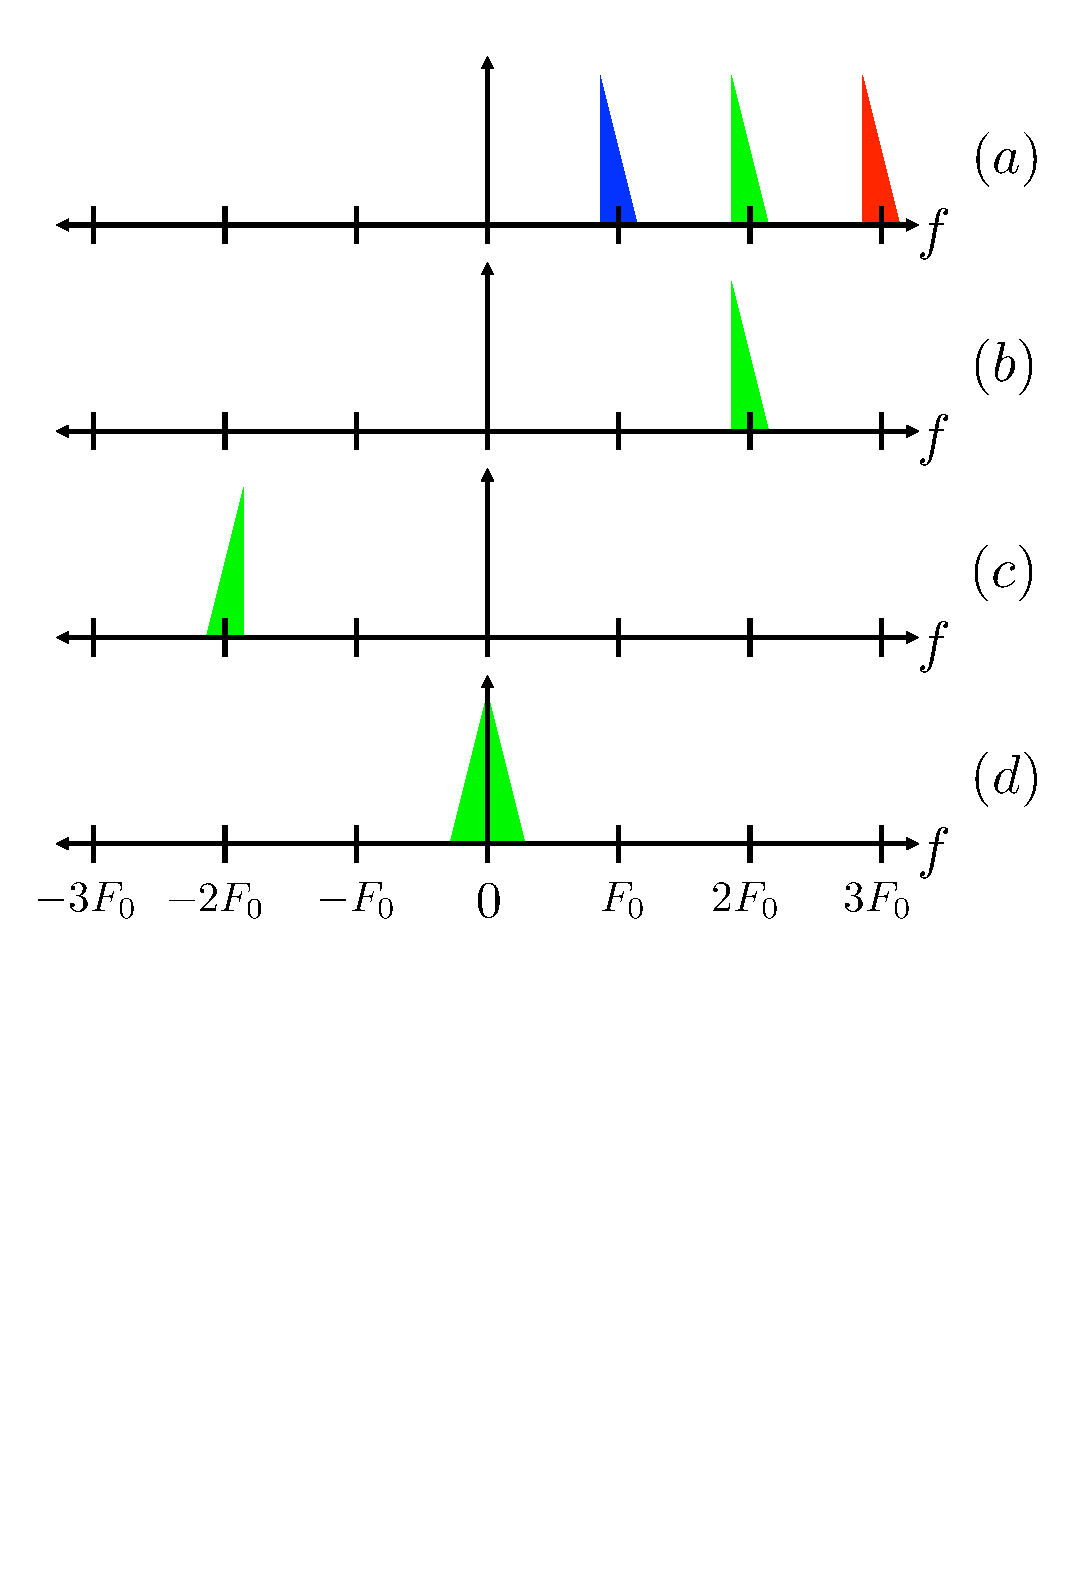
\includegraphics[width=.62\textwidth]{harmonic_envelope}   
        \caption{Magnitude of spectrum for equations \ref{eq:harmonic_envelope_spectrum_a} through \ref{eq:harmonic_envelope_spectrum_d}}
%        \caption{$(a) | \widehat{X}[n,f) |$
%    				$(b) | \widehat{X}_1[n,f) |$
%				$(c) | \widehat{X}_1^*[n,-f) |$
%				$(d) | \widehat{X}_1[n,f) * \widehat{X}_1^*[n,-f) |$}
\end{figure}

The envelope can always be acquired from the squared envelope by a final square root operation.  This operation introduces nonlinearities at multiples of $F_0$ that are difficult to analyze.  For mathematical convenience, during our analysis we can consider the squared envelope.  This final square root operation will remain constant across all examples which allows us to not consider it.

\begin{align}
\label{eq:square_root_relationship}
m_1[n] = \Big|\widehat{x}_1[n]\Big| = \Big[ \widehat{x}_1[n] \widehat{x}_1^*[n] \Big]^\frac{1}{2}
\end{align}

\subsection{Estimated Envelope}

Let's now evaluate our estimate, using equation~\ref{eq:envelope_extraction}.  As stated above, we consider the squared envelope.

\begin{align}
\tilde{m}_k^2[n] =& \Big| \widehat{x}[n]e^{-j \omega_kn} * h_k[n]]  \Big|^2 \nonumber \\
%
=& \Bigg|  \sum\limits_{l=0}^K m_l[n]e^{j(\theta_l[n] - \omega_k[n])}*h_k[n] \Bigg|^2 \nonumber \\
%
\approx& \Bigg|  \sum\limits_{l=0}^K m_l[n] \Big(e^{j(\theta_l[n] - \omega_k[n])}*h_k[n] \Big) \Bigg|^2 \nonumber \\
%
=& \Bigg|  \sum\limits_{l=0}^K m_l[n] e^{j(\omega_{k,l}n + \phi_k)} H_k\big(e^{j\omega_{k,l}}\big) \Bigg|^2 \\
%
\label{eq:downshift_radian_frequency}
\omega_{k,l} =& 2\pi\frac{(l+1)F_0 - F_{ds,k}}{F_s} \\
%
h_k[n] \Longleftrightarrow& H_k\big(e^{j\omega}\big)
\end{align}

$\omega_{k,l}$ is the downshift of the $l$'th harmonic for the estimate of the $k$'th envelope.  $H_k\big(e^{j\omega}\big)$ is the discrete Fourier transform (DFT) of $h_k[n]$.

Expanding this equation we get:

\begin{align}
\tilde{m}_k^2[n] =& \sum\limits_{l=0}^K \sum\limits_{i=0}^K m_l[n] m_i^*[n] e^{j(l-i)F_0} H_k\big(e^{j\omega_{k,l}}\big)H_k^*\big(e^{j\omega_{k,i}}\big) \\
%
%
%
=& \sum\limits_{l=0}^K \Big|m_l[n]\Big|^2 \Big|H_k\big(e^{j\omega_{k,l}}\big)\Big|^2 \nonumber \\
%
%
+& e^{-j2\pi \frac{F_0}{Fs}n} \sum\limits_{l=0}^{K-1} m_l[n] m_{l+1}^*[n] H_k\big(e^{j\omega_{k,l}}\big)H_k^*\big(e^{j\omega_{k,l+1}}\big) \nonumber \\
%
+&  e^{j2\pi \frac{F_0}{Fs}n} \sum\limits_{l=1}^{K} m_l[n] m_{l-1}^*[n] H_k\big(e^{j\omega_{k,l}}\big)H_k^*\big(e^{j\omega_{k,l-1}}\big) \nonumber \\
%
%
+& e^{-j2\pi \frac{2F_0}{Fs}n} \sum\limits_{l=0}^{K-2} m_l[n] m_{l+2}^*[n] H_k\big(e^{j\omega_{k,l}}\big)H_k^*\big(e^{j\omega_{k,l+2}}\big) \nonumber \\
%
+& e^{j2\pi \frac{2F_0}{Fs}n}  \sum\limits_{l=2}^{K} m_l[n] m_{l-2}^*[n] H_k\big(e^{j\omega_{k,l}}\big)H_k^*\big(e^{j\omega_{k,l-2}}\big) \nonumber \\
%
%
+& ... \nonumber \\
%
%
+& e^{-j2\pi \frac{KF_0}{Fs}n} m_0[n] m_K^*[n] H_k\big(e^{j\omega_{k,0}}\big)H_k^*\big(e^{j\omega_{k,K}}\big) \nonumber \\
%
+& e^{j2\pi \frac{KF_0}{Fs}n}  m_K[n] m_0^*[n] H_k\big(e^{j\omega_{k,K}}\big)H_k^*\big(e^{j\omega_{k,0}}\big)
\end{align}

We can now think of $\tilde{m}_k[n]$ as a combination of terms each centered at $iF_0$ where the magnitude of each term is:

\begin{align}
\Big| \tilde{m}_{k,iF_0}[n] \Big| =& \Bigg[ \sum\limits_{l=0}^{K-|i|} \Big| m_l[n]\Big| \Big|m_{l+i}[n]\Big| \Big|H_k\big(e^{j\omega_{k,i}}\big)\Big| \Big|H_k\big(e^{j\omega_{k,l+i}}\big)\Big|\Bigg]^\frac{1}{2}, \quad -K \leq i \leq K \\
%
\Big| \tilde{m}_{k,0F_0}[n] \Big| =& \Bigg[  \sum\limits_{l=0}^K \Big|m_l[n]\Big|^2 \Big|H_k\big(e^{j\omega_{k,l}}\big)\Big|^2 \Bigg]^\frac{1}{2}
\end{align}

\subsection{3 Harmonic Example: Estimated Envelope}

Let's go back to our three harmonic example.  We are again trying to acquire the 1st harmonic, $m_1[n]$ (green).  We define $\omega_1 = 2F_0$.

\begin{figure}[!ht]
\label{fig:harmonic_envelope_estimate}
  \centering
    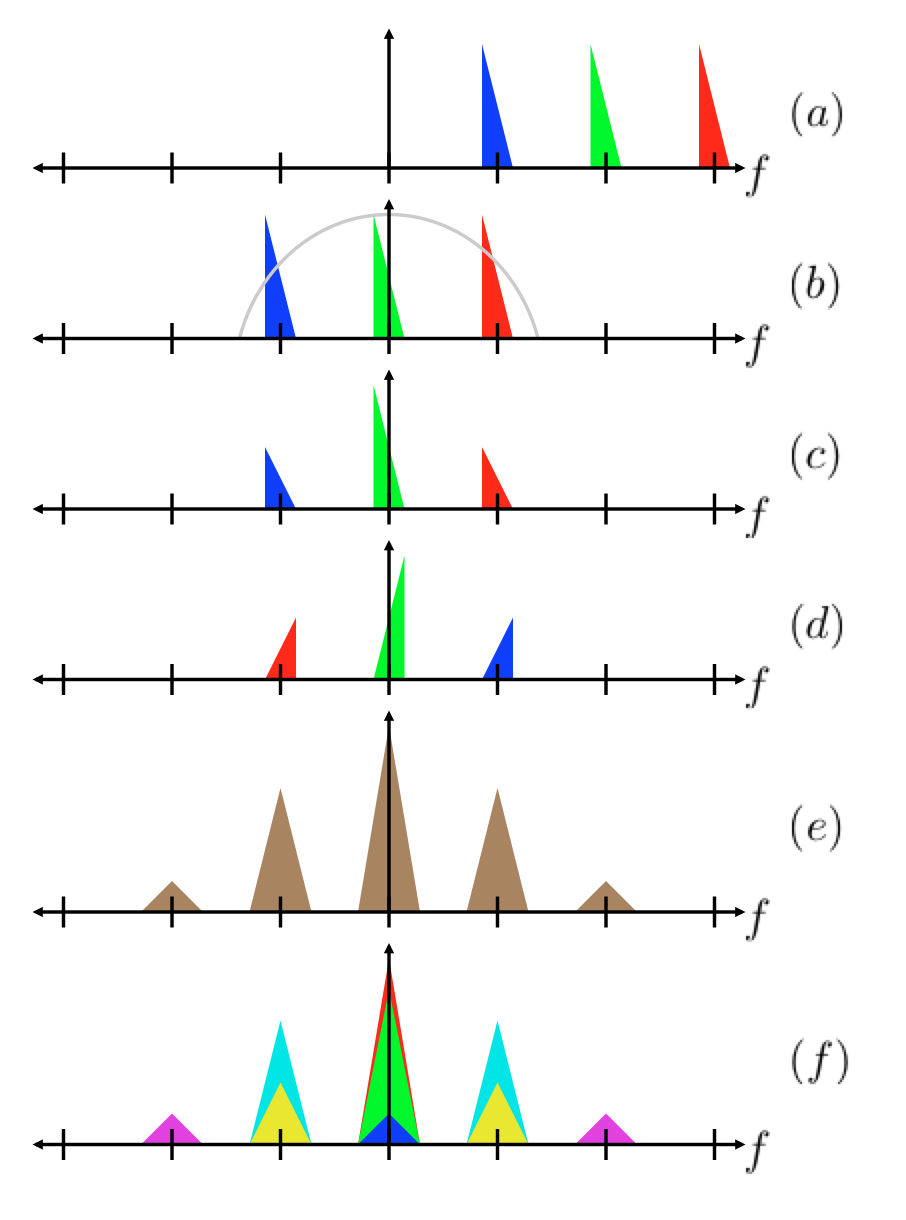
\includegraphics[width=.62\textwidth]{harmonic_envelope_estimate}   
    \caption{$(a) | \widehat{X}[n,f) |$   
    				$(b) | \widehat{X}[n,f - 2F_0) |$  
				$(c) | \widehat{X}[n,f - 2F_0) | | H_1(f) |$
				$(d) | \widehat{X}^*[n,-f + 2F_0) | | H_1(-f) |$
				$(e) | \mathcal{F} \{ \tilde{m}_1^2[n] \} |$
				$(f)$ contributions of separate components of $(e)$}
\end{figure}

We can see the relationships

\begin{align}
\widehat{x}[n] \Longleftrightarrow& \widehat{X}[n,f) \\
\widehat{x}[n]e^{-j2\pi \frac{2F_0}{F_s}n} \Longleftrightarrow& \widehat{X}[n,f - 2F_0) \\
\widehat{x}[n]e^{-j2\pi \frac{2F_0}{F_s}n} * h_2[n] \Longleftrightarrow& \widehat{X}[n,f - 2F_0) H_1(f) \\
\tilde{m}_1^2[n] \Longleftrightarrow& \widehat{X}[n,f - 2F_0) H_1(f) * \widehat{X}^*[n,-f + 2F_0) H_1^*(-f)
\end{align}

The interesting part of figure~\ref{fig:harmonic_envelope_estimate} is $(f)$.  We see our green component that we were looking for, however there are a whole lot of other things that we didn't want.

Figure~\ref{fig:harmonic_envelope}$(d)$ is equivalent to the green component of  figure~\ref{fig:harmonic_envelope_estimate}$(f)$ if our filter $|H_1(f)| = 1$ when $f \approx 0$.

The other components come from interactions with the unwanted harmonics that we failed to completely filter out.  For clarity the convolution is visualized in figures \ref{fig:harmonic_envelope_2F0}, \ref{fig:harmonic_envelope_F0}, \ref{fig:harmonic_envelope_0}.  Positive and negative components are mirror images so the positive components are not explicitly visualized.

\begin{figure}[!ht]
   \centering
   \label{fig:harmonic_envelope_2F0}
    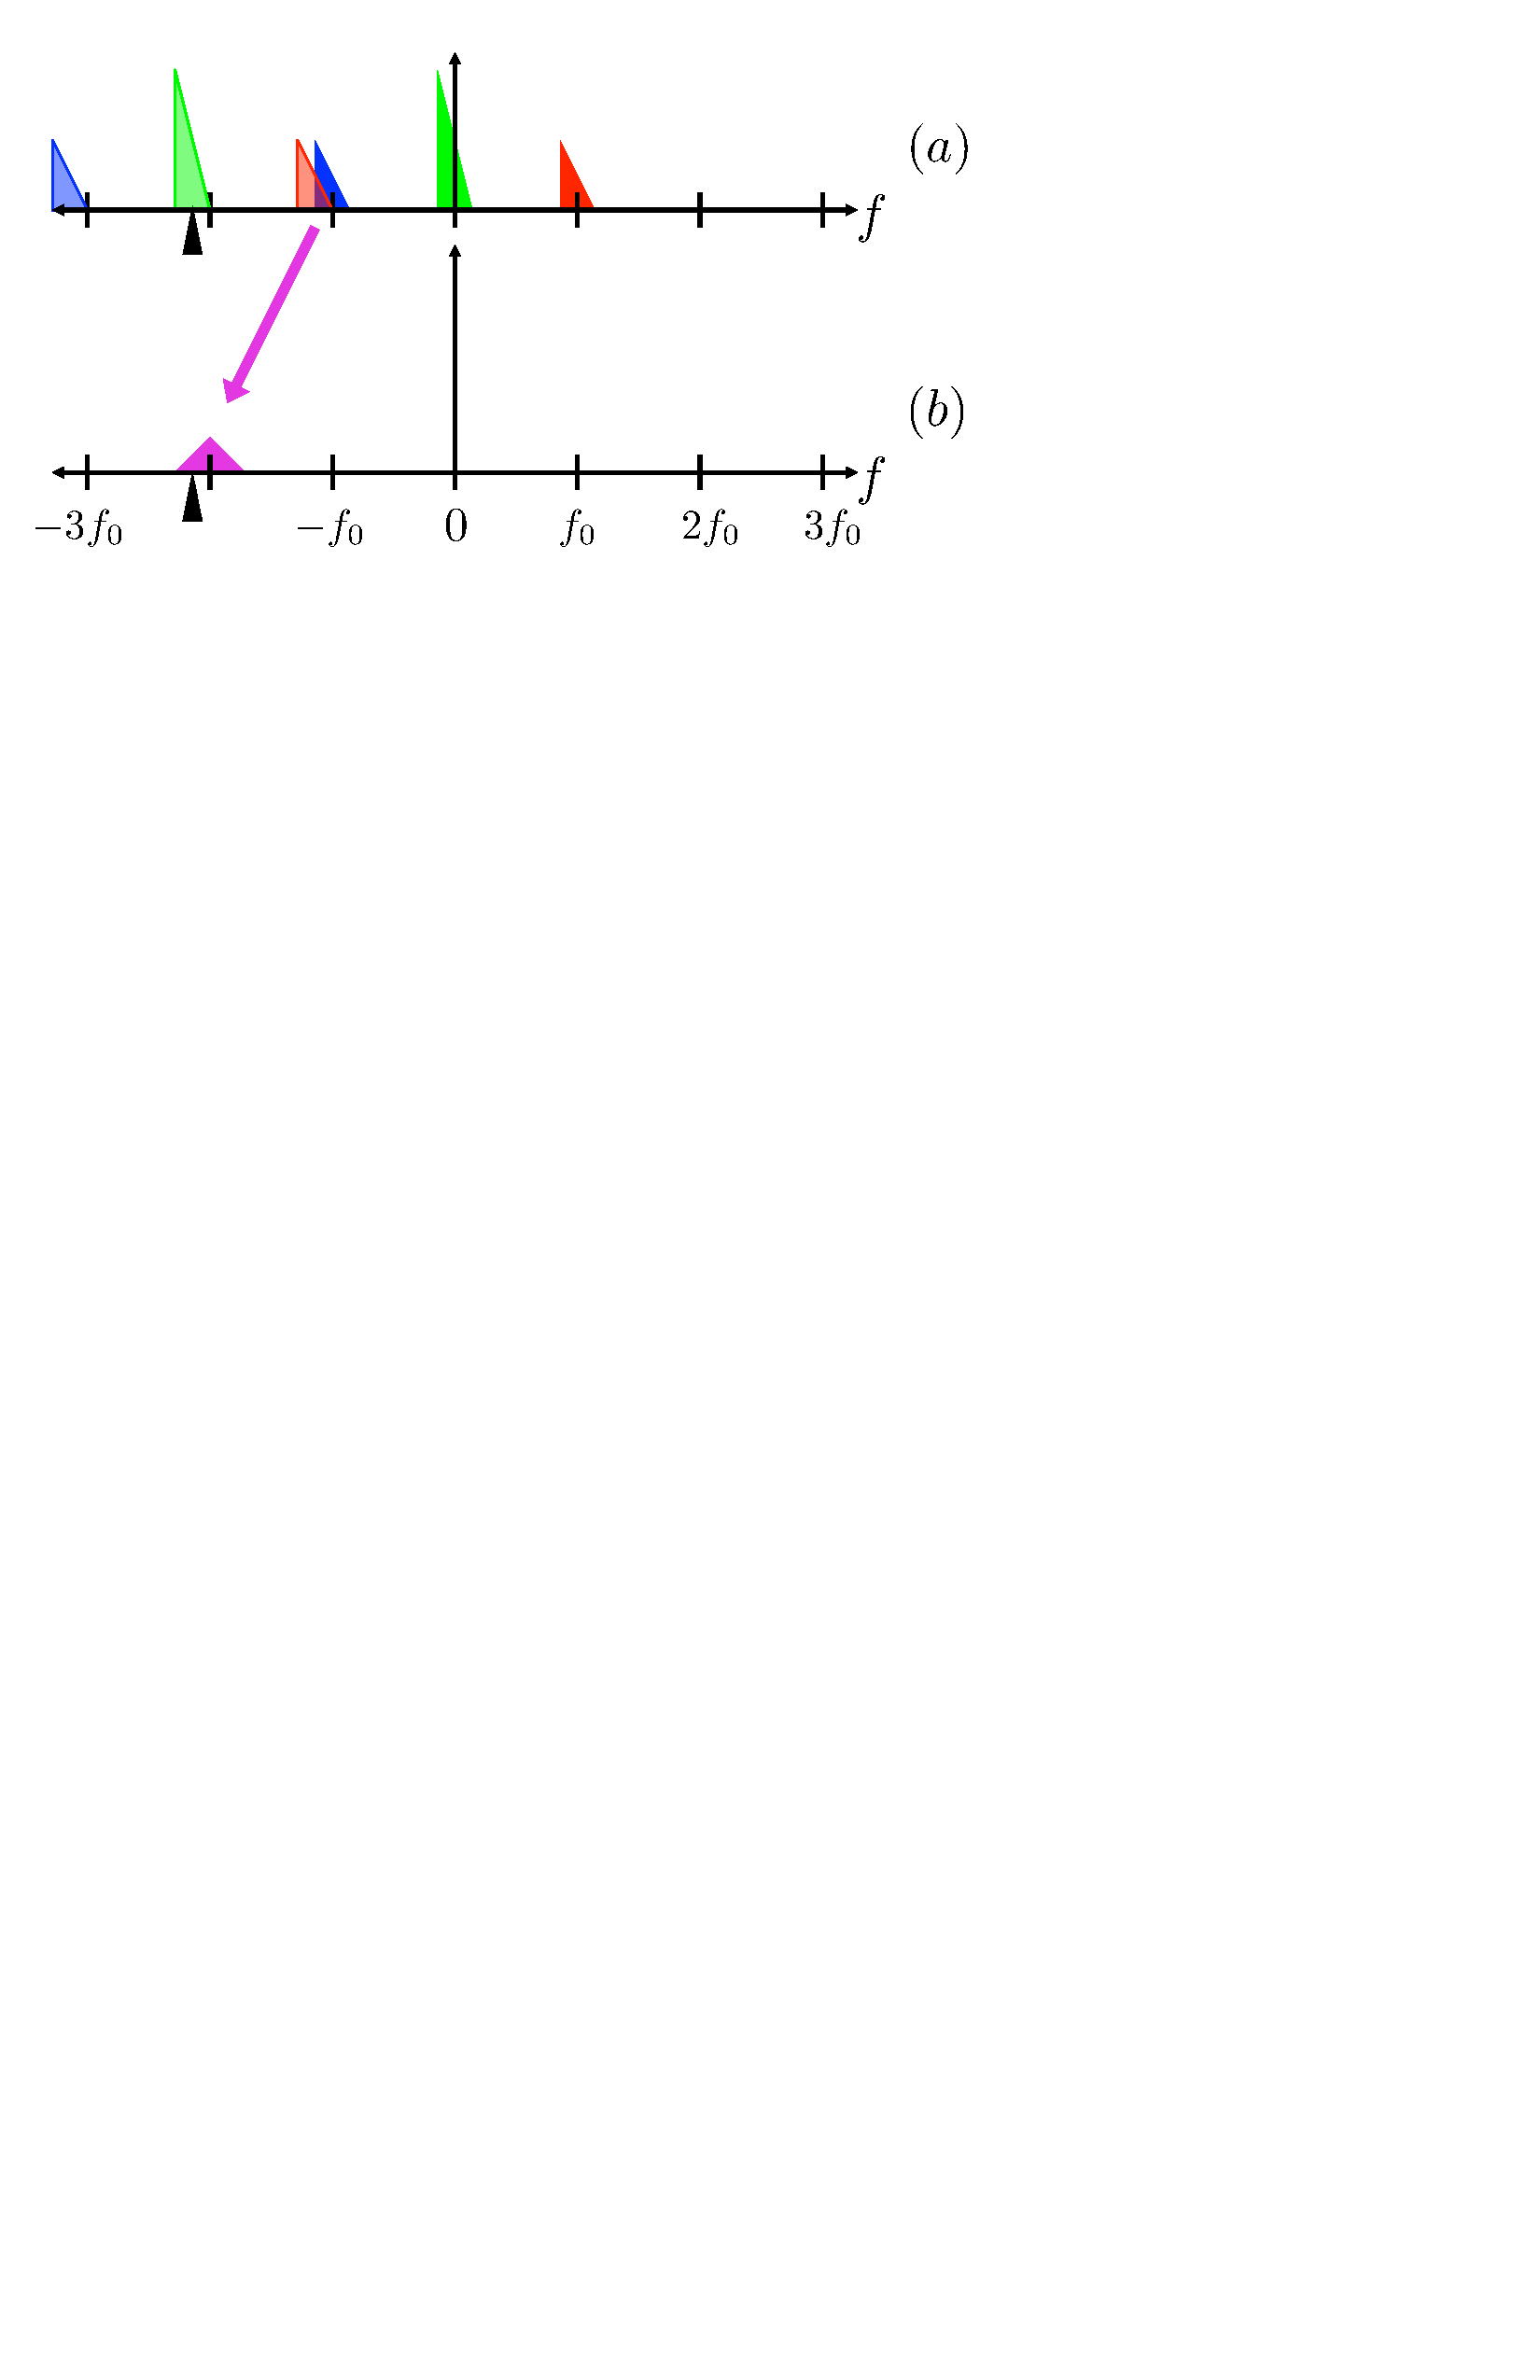
\includegraphics[width=.62\textwidth]{harmonic_envelope_2F0}   
    \caption{Envelope Estimate $-2F_0$ Component}
    \label{fig:harmonic_envelope_F0}
    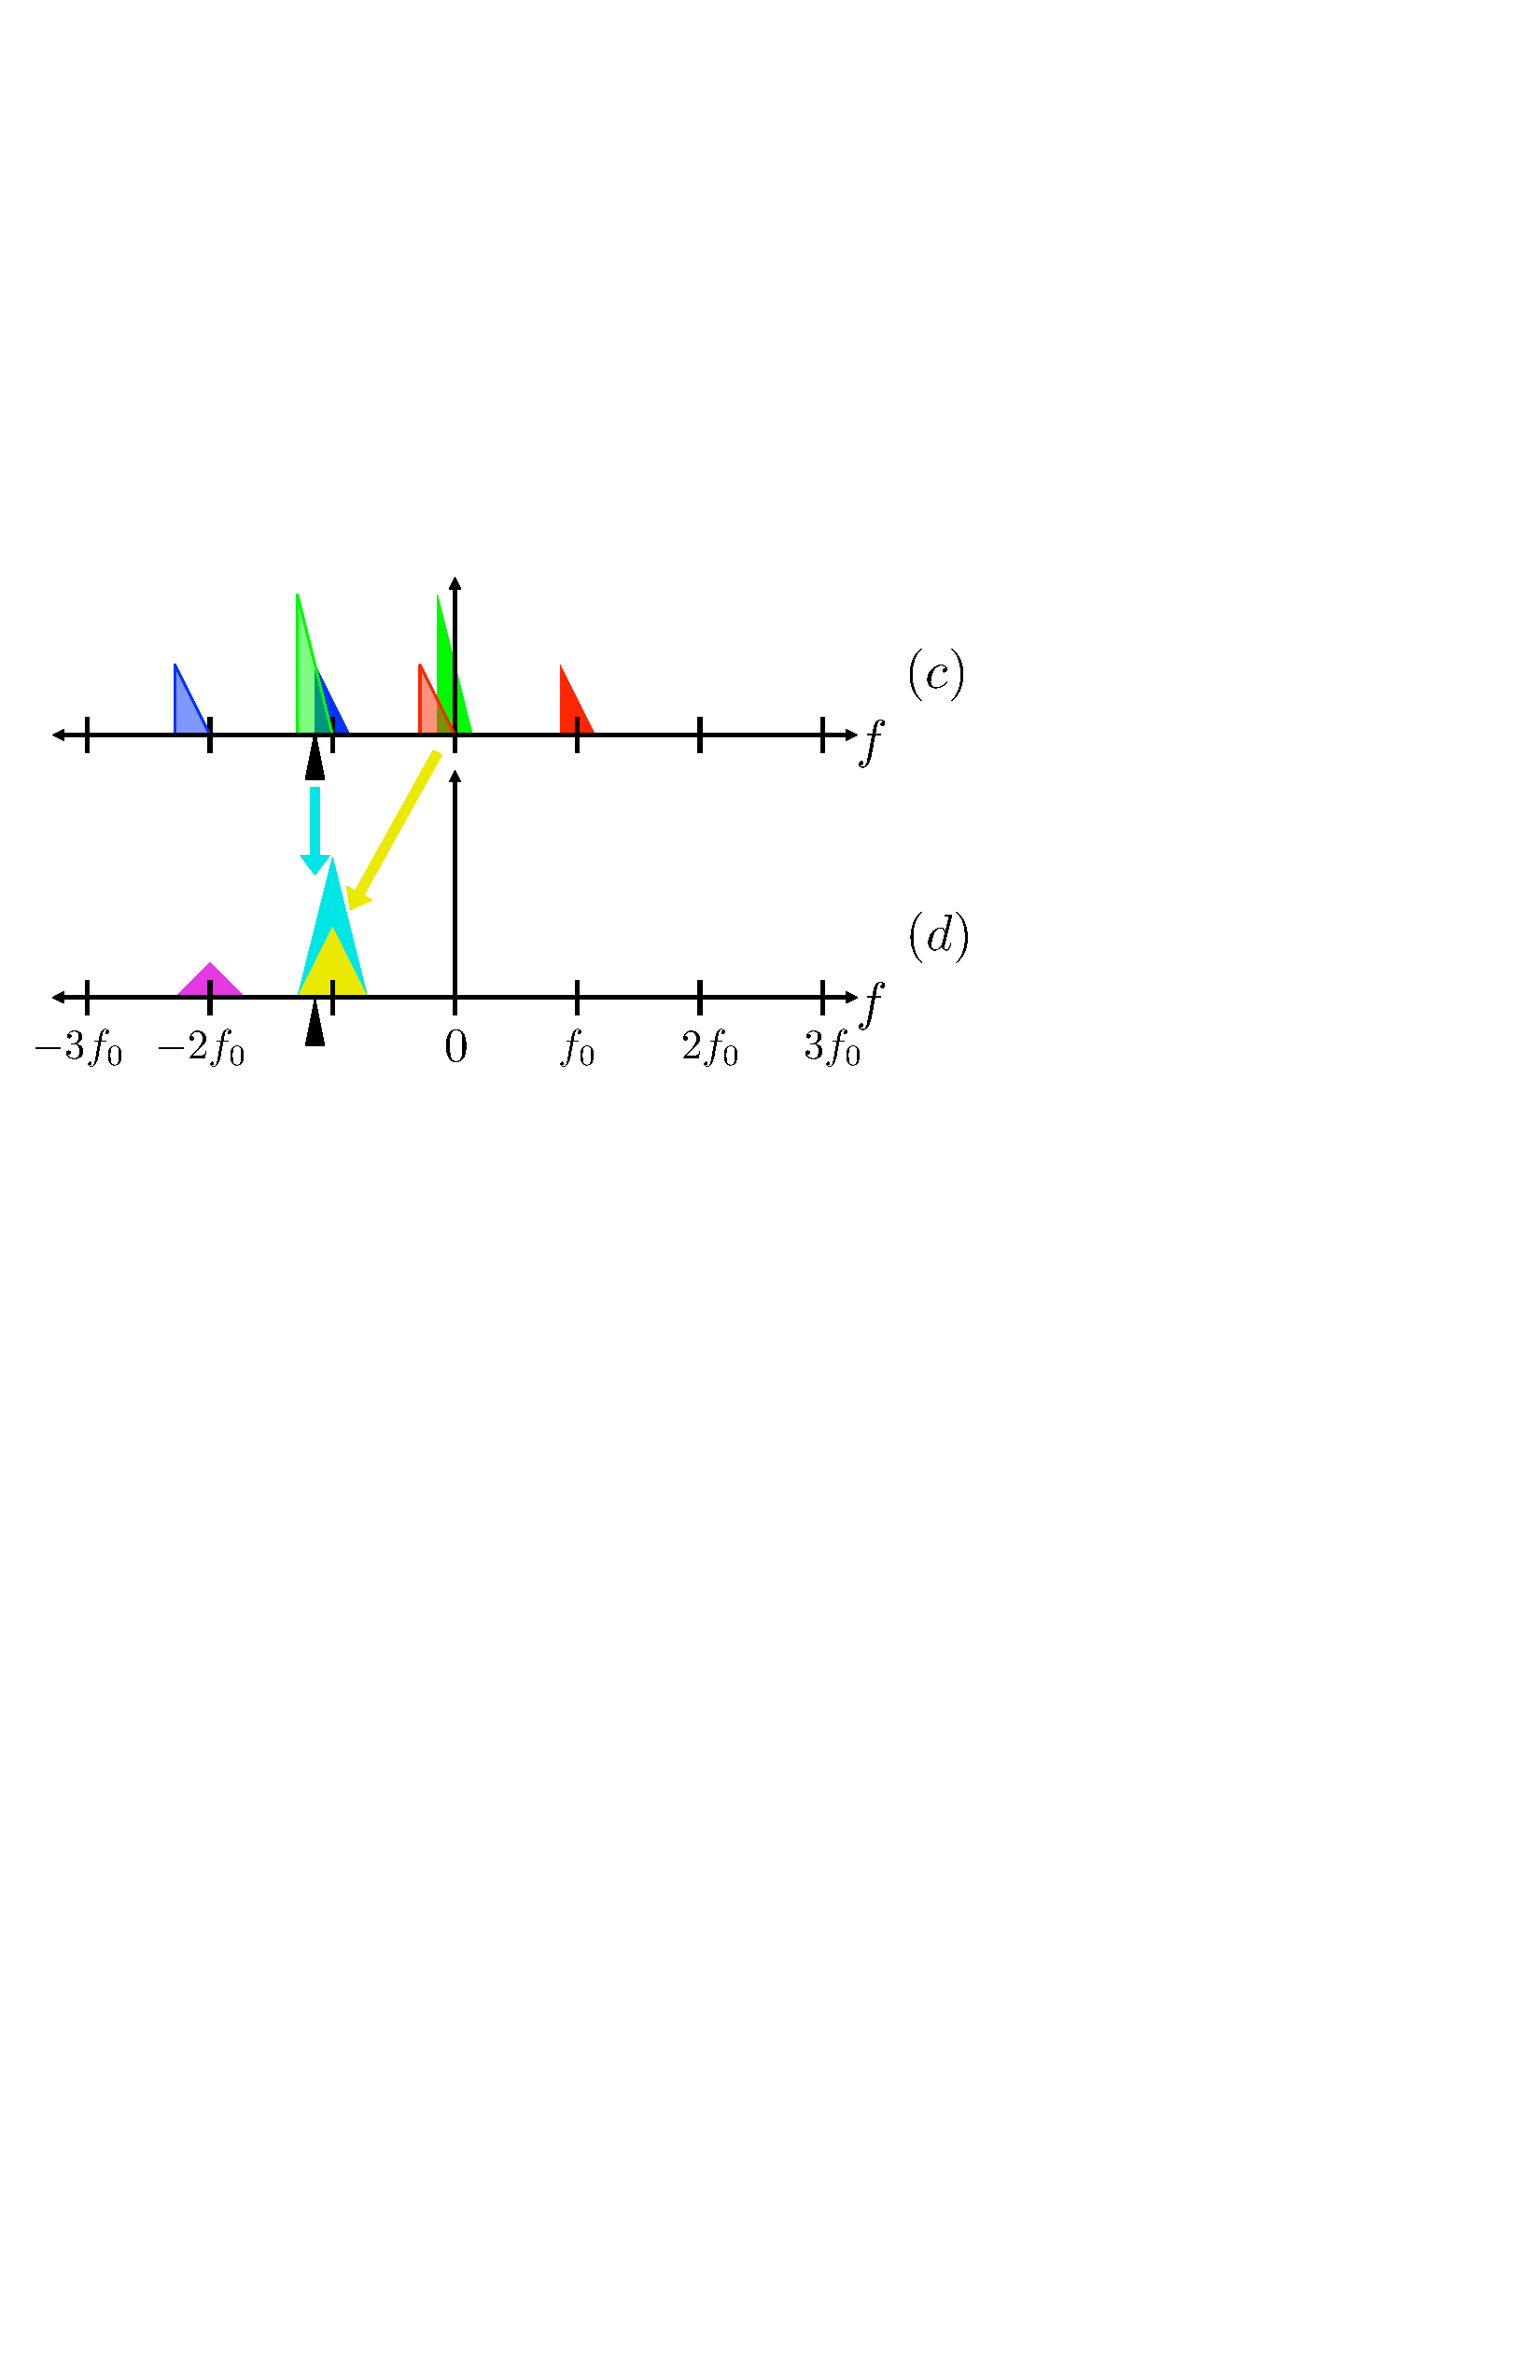
\includegraphics[width=.62\textwidth]{harmonic_envelope_F0} 
    \caption{Envelope Estimate $-F_0$ Component}
    \label{fig:harmonic_envelope_0}
    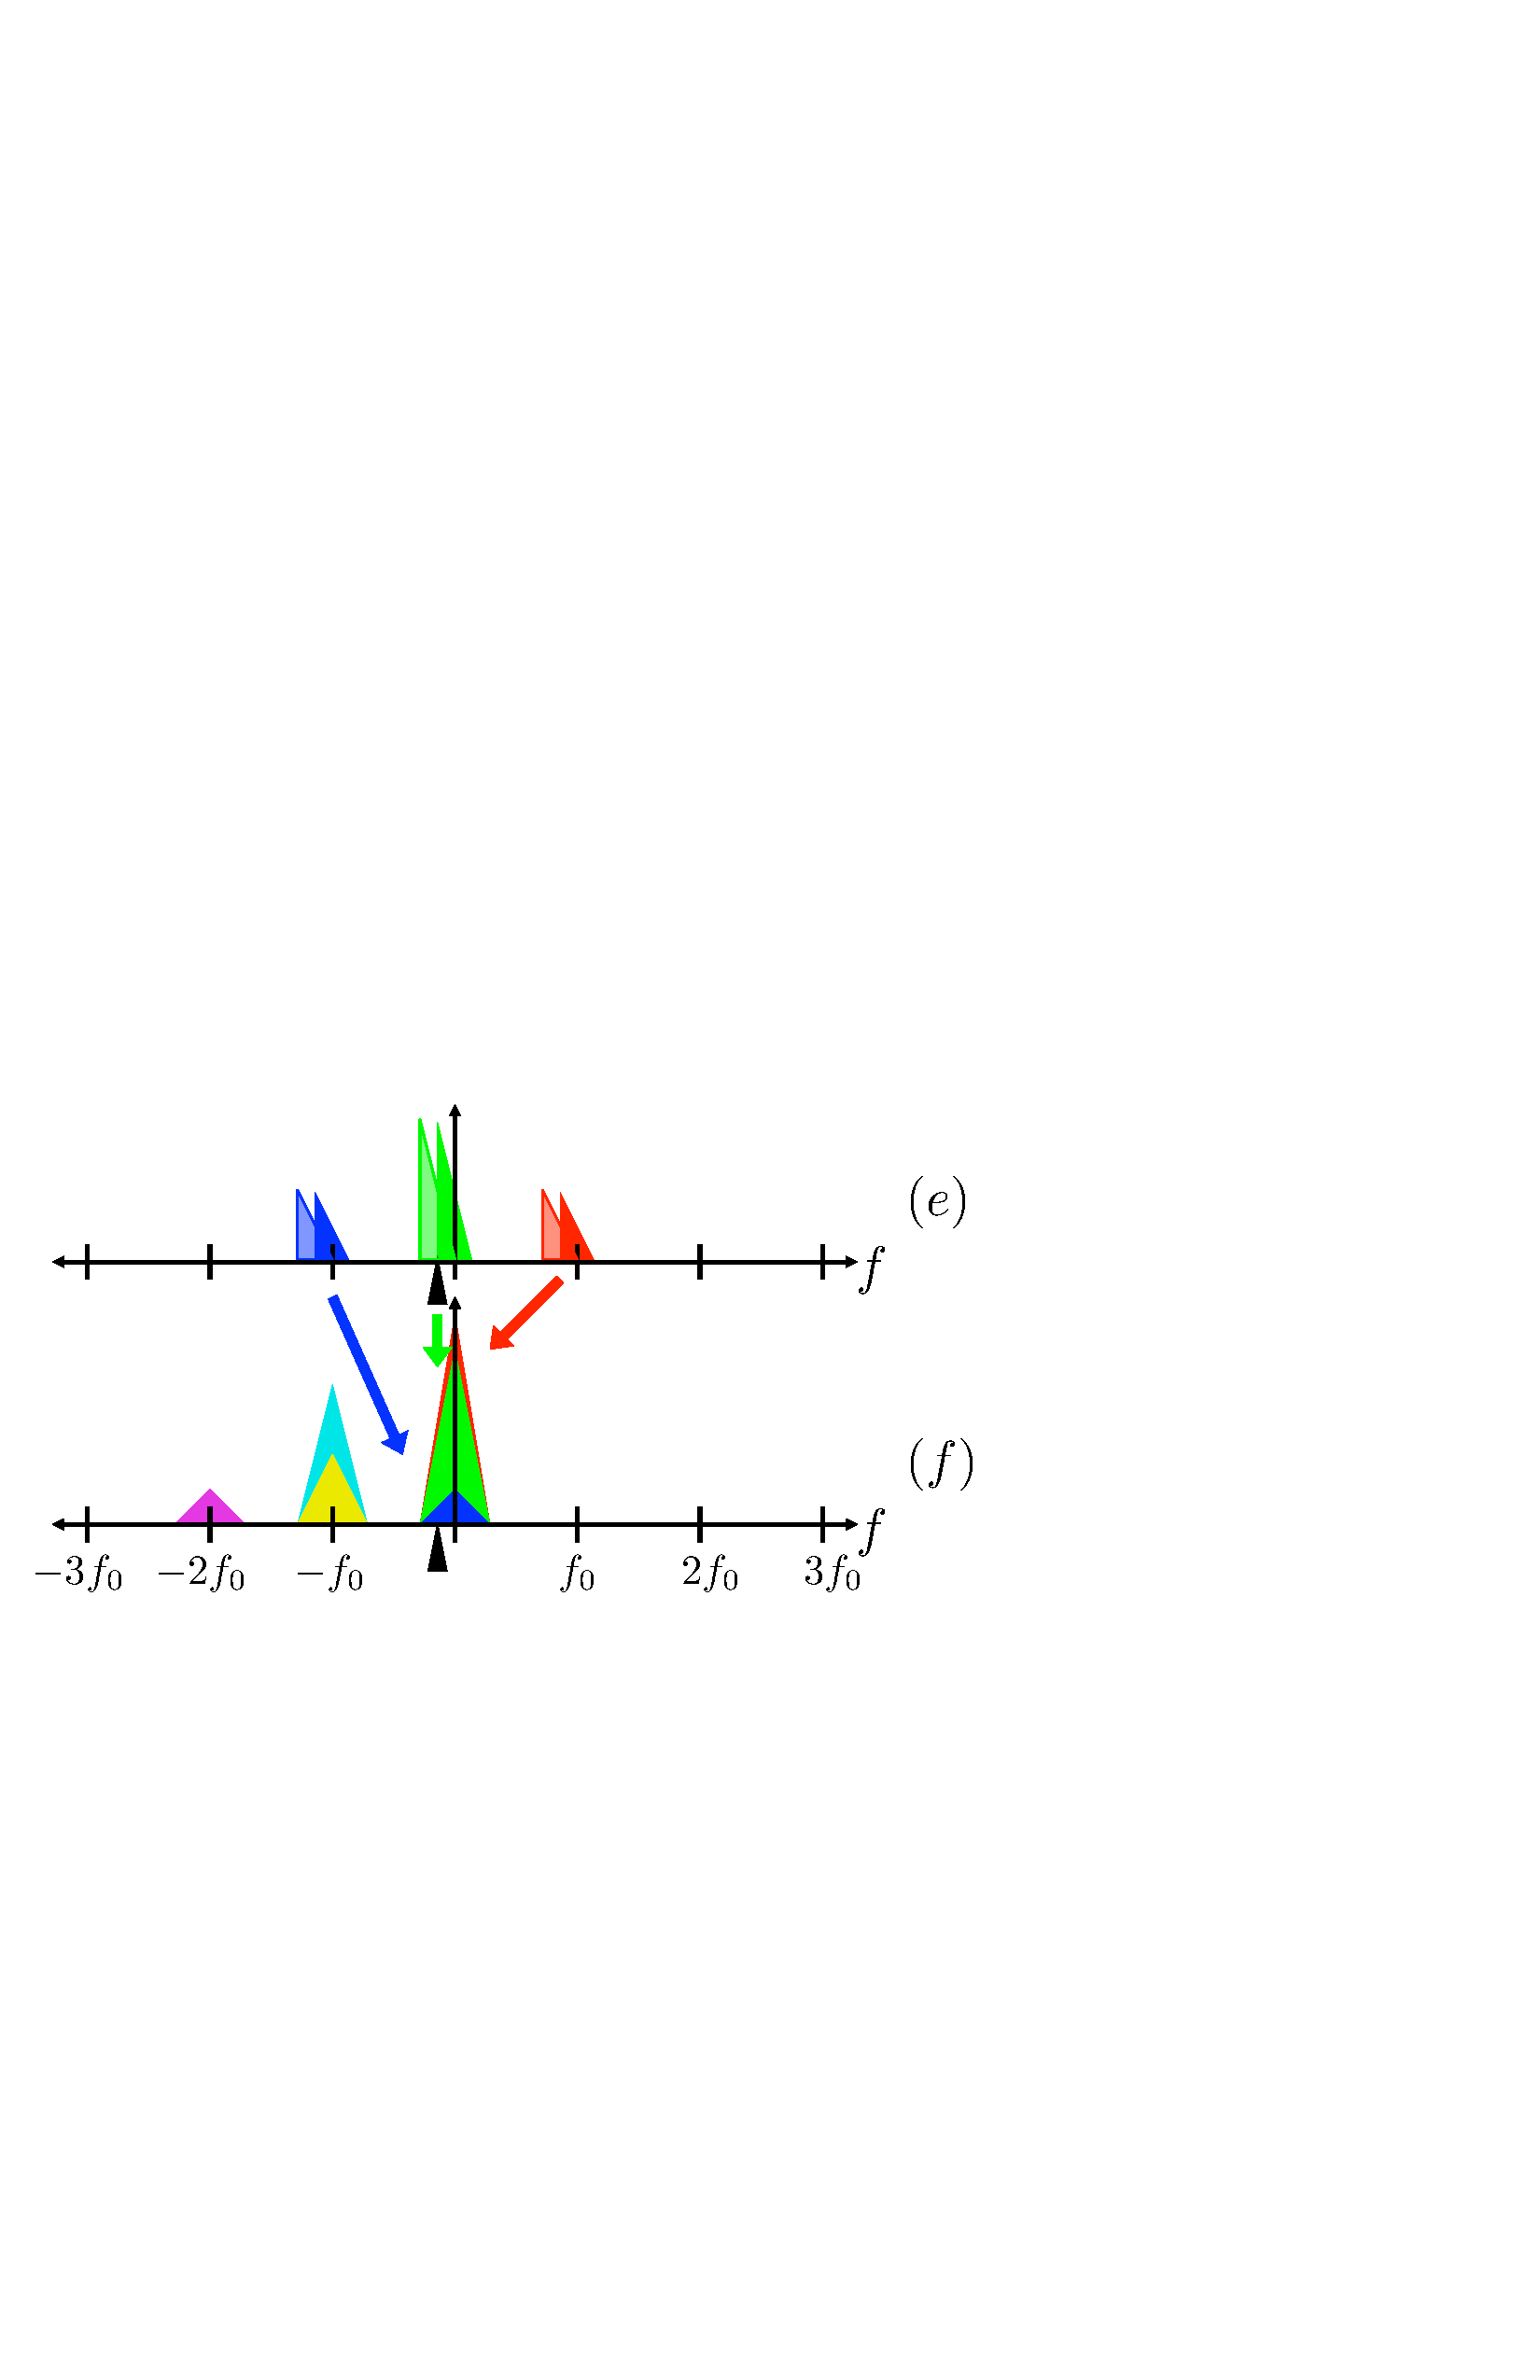
\includegraphics[width=.62\textwidth]{harmonic_envelope_0}
    \caption{Envelope Estimate Baseband Component}
\end{figure}

\section{Steady-State Metrics}

In considering how well our envelope $\tilde{m}_k[n]$ estimates $m_k[n]$ there are three important metrics.  We will now discuss each in detail.

\subsection{Coherent Gain}

Coherent gain is defined as the gain of the harmonic of interest, $k$.

\begin{align}
G_k = \Big| H_k\big(e^{j\omega_{k,k}}\big) \Big|
\end{align}

Recalling equation~\ref{eq:downshift_radian_frequency}, if $F_{ds,k} = (k+1)F_0$ then, $w_{k,k} = 0$ and the coherent gain is simply the DC gain of the filter.

\begin{align}
G_k = \Big| H_k(0) \Big| = \sum_n h_k[n]
\end{align}

We may further simplify this by normalizing our filter such that $\Big| H_k(0) \Big| = 1$.  Of course, our downshift frequency won't be ideal in real systems.  Factors to consider include the quantization of $F_{ds,k}$ and the accuracy of $F_0$ estimation.

\subsection{Harmonic SIR}

Continuing our focus on the baseband, another question is: what is the contribution of the target harmonic versus the others?  The baseband component is contributed to by spectral leakage due to non-ideal filters.  This is visualized as the red and blue in figure~\ref{fig:harmonic_envelope_estimate}$(f)$.  The harmonic signal-to-interference-ratio (SIR) quantifies the ratio of target harmonic to spectral leakage.

\begin{align}
SIR_k =& \frac{\Big| H_k\big(e^{j\omega_{k,k}}\big) \Big|} {\Bigg[ \sum\limits_{l=0}^K \Big|H_k\big(e^{j\omega_{k,l}}\big)\Big|^2 \Bigg] ^ \frac{1}{2}}
\end{align}

The terms will roll off as the harmonic center frequencies get further away from $F_{ds,k}$, so typically $SIR_k$ is sufficiently described by only one or two harmonics on either side of the $k$'th, i.e. $k-2 \leq l \leq k+2$.

Harmonic SIR does not describe the true signal-dependent SIR, as varying envelope magnitudes across harmonics will change this, however it does provide an objective measure of the quality of our system to arbitrary harmonic inputs.

% one measure of spectral leakage is asymptotic falloff (db/octave) of sidelobes [windows for harmonic analysis]

\subsection{Modulation Depth}

Finally, we consider the magnitude of each bandpass component relative to baseband.  These terms appear in our envelope estimate as modulations at rates that are multiples of $F_0$.  Because of the forced symmetry of the real envelope we only need to consider positive frequencies, $iF_0$.

\begin{align}
D_{k,i} =& \frac{\Bigg[ \sum\limits_{l=0}^{K-i} \Big|H_k\big(e^{j\omega_{k,l}}\big)\Big| \Big|H_k\big(e^{j\omega_{k,l+i}}\big)\Big|\Bigg]^\frac{1}{2}}
{\Bigg[ \sum\limits_{l=0}^K \Big|H_k\big(e^{j\omega_{k,l}}\big)\Big|^2 \Bigg] ^ \frac{1}{2}}, \quad 1 \leq i \leq K
\end{align}

The largest value and, for that reason, most important value is $D_{k,1}$, the modulation depth at $F_0$.

\section{Explicit Temporal Modulation}

So our three metrics are coherent gain, harmonic SIR and modulation depth.  We aim for a coherent gain of $G_k = 1$, maximum possible SIR and one would think minimum modulation depth.

Interestingly, some current CI processing strategies such as ACE intentionally allow for induced modulations from non-isolated harmonics.  This provides a temporal cue to the user which plays into pitch percept.

The alternative is to use narrow enough filter cutoffs to eliminate these modulations, and then explicitly modulate the signal.  In this option we need further processing such as a pitch estimator to determine the modulation rate.

In this document we argue that the latter, explicit modulation option is better.  The reasoning is best shown by a motivational example.

Let's consider a single note played by two different instruments, clarinet and saxophone.  In this example $F_0 = 261Hz$.  The clarinet is interesting in that it only has energy at odd harmonics.

We attempt to estimate the 3rd harmonic, $m_3[n]$.  We first downshift by $-3F_0$, then lowpass filter.  The spectrum of each signal at this stage is visualized in figure~\ref{fig:clarinetVSsax_F}.  The top panel shows the output of a sufficiently narrow filter where the 3rd harmonic is isolated.  The bottom panel shows a different filter design that intentionally allows the two adjacent harmonics to pass through.  Here we start to see the problem, that despite the wide bandwidth filter, there is no energy around $\pm F_0$ for the clarinet because of the harmonic structure.

\begin{figure}[!ht]
\label{fig:clarinetVSsax_F}
  \centering
    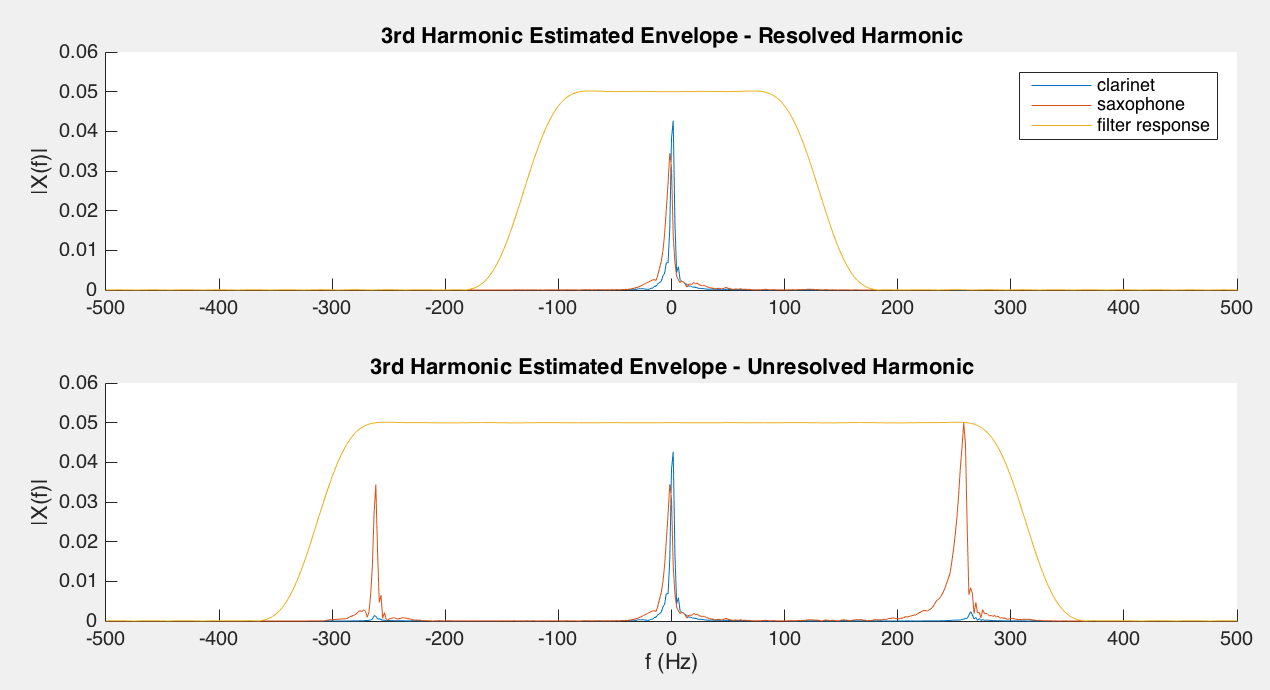
\includegraphics[width=1\textwidth]{clarinetVSsax_F}
    \caption{Clarinet vs Saxophone Harmonic Components}
\end{figure}

Figure~\ref{fig:clarinetVSsax_T} shows the time-domain envelopes resulting from this processing.  The input signals were normalized such that the top panel shows the same signal power for both instruments.

The problem is clearly represented in the bottom panel, were we have a very large $F_0$ modulation in the saxophone envelope but little to no change in the clarinet.  The result is that we have a much stronger temporal pitch cue as well as louder overall volume to the saxophone.

\begin{figure}[!ht]
\label{fig:clarinetVSsax_T}
  \centering
    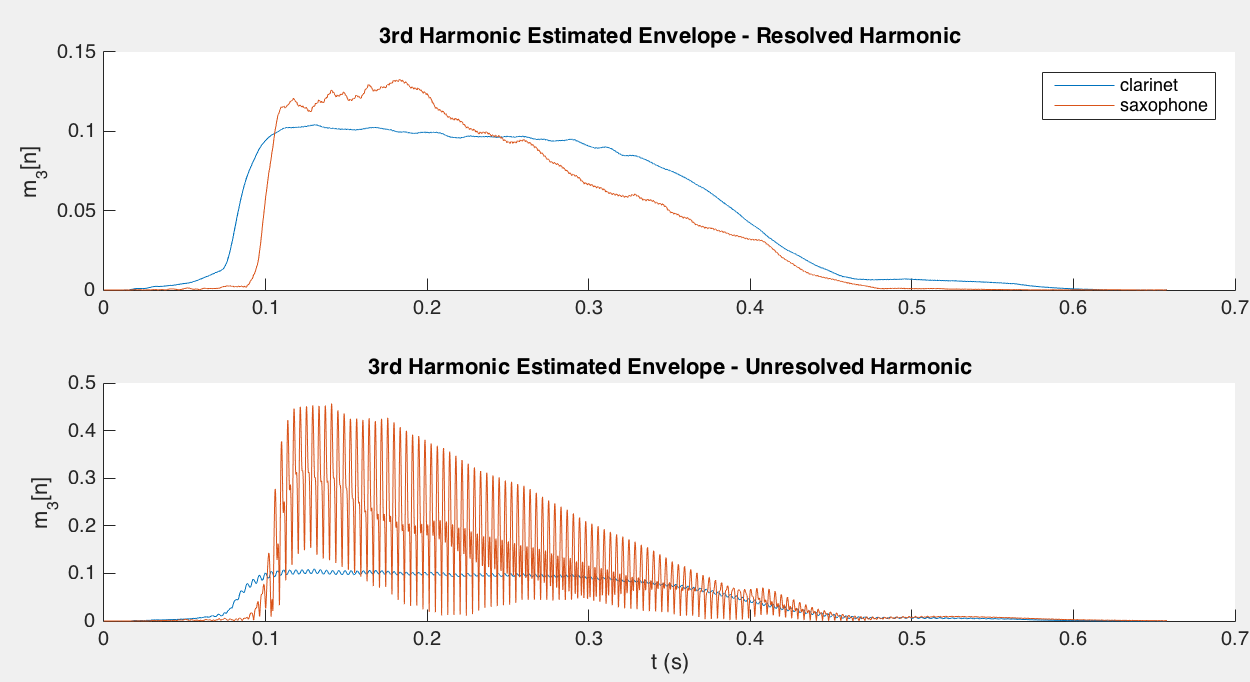
\includegraphics[width=1\textwidth]{clarinetVSsax_T}   
    \caption{Clarinet vs Saxophone Envelope Estimates}
\end{figure}

Spectral leakage into other harmonic envelopes is not natural.  It forces the envelope to modulate as a function of the adjacent harmonics which, as we just saw, is signal dependent.  Furthermore, if we have uniform bandwidth filters, (as ACE does), the harmonic resolution will not behave as it does in the cochlea.

Beyond this example, explicit modulation decouples $F_0$ and modulation depth.  This way we have much more control over modulation depth while still making optimal design decisions for envelope extraction.  We can decide modulation depth as a function of how harmonic the signal is.  eTone [REF] uses a harmonic probability metric to do just that.

\subsection{Followup Filter}

Another thing to note is that regardless of downshift frequency, our harmonic envelope will always have it's energy centered at baseband and multiples of $F_0$.  An alternative way of eliminating induced modulations is to add a lowpass filter to the end of the processing chain.

There are a handful of research strategies [REF?] that have used this additional filter.  eTone's envelope follower is an example of this.

The main improvement to this method is that we can guarantee to eliminate modulations.  This could also be achieved by designing a sufficiently narrow filter, $h_k[n]$ however this brings about a tradeoff, where the narrower our filter is the more susceptible we are to error in downshift frequency.

In terms of our three metrics, the followup filter will provide us with a robust coherent gain and guaranteed low modulation depth at the cost of lower harmonic SIR.

Another point to consider is the cost of adding an additional processing stage.  The additional stage means more memory, clock cycles and processing delay.

% Because of transient smearing, we will not be using this method

\section{Steady-State Evaluation of Strategies}

\subsection{design parameters}

filter and downshift

ideally: 
BW = F0/2
downshift = exp(kF0)

downshift quantization, bandwidth as function of F, F0?

modulation depth (kind of another SIR) as a function of downshift quantization and filter

\subsection{figures}

\section{Transients}

quantify for best case and worst case where worst case is the fastest transient relevant to music (this should also hinge on CI limitations)

maximum onset dynamic range "90ms - 10ms = 80ms"
and ratio of filter smeared range to max range
rinse and repeat for CI's

\section{Changing F0}

dips due to quantization

\subsection{scalloping loss}

[windows for harmonic analysis]

scalloping loss or picket-fence effect, ratio of coherent gain for tone located half a bin from DFT sample point to coherent gain for tone located exactly at sample point

\begin{align}
scalloping loss = \frac{| H(\frac{1}{2} \frac{F_s}{N}) |}{H(0)}
\end{align}

"althought scalloping loss is useful, it's not entirely informative.  if the scalloping loss if high, then this relates to a sharp cutoff which is actually good for increasing purity of the harmonic"

worst case processing loss = scalloping loss * PL
where PL is reduced gain of window (which i have been canceling out)
**where does worst case processing loss fit in?**



ALL METRICS:

ENBW (accumulated noise)
PL (gain at DC)
PG (same as PL?)
scalloping loss (downshift quantization worst case)
worst case PL = PL*SL

harmonic SIR
harmonic gain (maybe not overly relevant due to AGC, etc)
					(how is it affected in a relative sense? worst vs best)
modulation depth (spectral leakage)
transients
changing F0 (scalloping loss dip only, and harmonic SIR)




\chapter{Efficient Interpolation Algorithm}

FFT with changeable window, and interpolate

Can this be done with different filter as function of F0?
We probably need to design the filters such that they pass reconstruction requirements

Is the actual equation just a sinc function times a phase shift?!

READ THIS: [An Intelligent FFT-Analyzer with Harmonic Interference Effect Correction and Uncertainty Evaluation]

\chapter{-----------------------------------}


% ========== Chapter 6

\chapter{Conclusion}

\section{Summary}

\section{Future Work}



%
% ==========   Bibliography
%
\nocite{*}   % include everything in the uwthesis.bib file
\bibliographystyle{plain}
\bibliography{ganter_thesis}
%
% ==========   Appendices
%
\appendix
\raggedbottom\sloppy
 
% ========== Appendix A
 
\chapter{Where to find the files}
 
The uwthesis class file, {\tt uwthesis.cls}, contains the parameter settings,
macro definitions, and other \TeX nical commands which
allow \LaTeX\ to format a thesis.  
The source to
the document you are reading, {\tt uwthesis.tex},
contains many formatting examples
which you may find useful.
The bibliography database, {\tt uwthesis.bib}, contains instructions
to BibTeX to create and format the bibliography.
You can find the latest of these files on:

\begin{itemize}
\item My page.
\begin{description}
\item[] \verb%http://staff.washington.edu/fox/tex/uwthesis.html%
\end{description}

\item CTAN
\begin{description}
\item[]  \verb%http://tug.ctan.org/tex-archive/macros/latex/contrib/uwthesis/%
\item[]  (not always as up-to-date as my site)
\end{description}

\end{itemize}

\vita{Jim Fox is a Software Engineer with UW Information Technology at the University of Washington.
His duties do not include maintaining this package.  That is rather
an avocation which he enjoys as time and circumstance allow.

He welcomes your comments to {\tt fox@uw.edu}.
}


\end{document}
